\documentclass{article}
\usepackage[utf8]{inputenc}
\usepackage[spanish]{babel}
\usepackage{listings}
\usepackage{graphicx}
\graphicspath{ {images/} }
\usepackage{cite}

\begin{document}

\begin{titlepage}
    \begin{center}
        \vspace*{1cm}
            
        \Huge
        \textbf{LA MEMORIA DEL COMPUTADOR}
            
        \vspace{0.5cm}
        \LARGE
        Un recurso informático invaluable.
        \vspace{1.5cm}
            
        \textbf{Julian Guillermo Zapata Rugeles}
            
        \vfill
            
        \vspace{0.8cm}
            
        \Large
        Despartamento de Ingeniería Electrónica y Telecomunicaciones\\
        Universidad de Antioquia\\
        Medellín\\
        Septiembre de 2020
            
    \end{center}
\end{titlepage}

\tableofcontents

\section{¿ Qué es la memoria de un computador ?}
Para conocer qué es la memoria de un computador debemos preguntarnos cómo funciona, un ejemplo práctico es imaginarnos un pequeño recipiente que es capaz de almacenar una carga eléctrica por un breve periodo de tiempo. El comportamiento físico de nuestro 'recipiente' que en electrónica se llama condensador(pues es capaz de almacenar energía sustentando un campo eléctrico) nos permite representar dos estados. Cuando nuestro recipiente está lleno (un nivel máximo de electrones) y cuando está vacío (ausencia de un mínimo de electrones), sin embargo esto no es suficiente para darnos una idea clara de como funciona la memoria.
Para entender este nuevo concepto es necesario bajar en las capas de abstracción para imaginar que nuestros recipientes pueden agruparse en bloques, supongamos unos 8 recipientes por bloque (a este bloque lo llamaremos byte) y estos pueden tener algún estado de los expuestos anteriormente. Eso significa que podemos tener 2 posibles estados elevado a la octava potencia (pues tenemos 8 recipientes).


\begin{figure}[h]
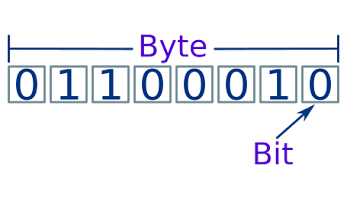
\includegraphics[width=3cm]{images/byte.png}
\centering
\caption{8 bits (8 recipientes)  agrupados en un bloque llamado byte. fuente imagen https://terminosaudiovisuales.es/byte/}
\label{fig:byte}
\end{figure}
\[2^{8}=256 \]
De manera abstracta podemos pensar en que cada número entre los 256 que se pueden obtener tras combinar los dos estados. Pueden representar 
 análogamente una letra, número o símbolo de nuestro alfabeto. La disposición de millones de bloques de nuestros recipientes pueden almacenar muchísimas representaciones abstractas de nuestro vocabulario y más.
Inmediatamente nos surge una pregunta qué a veces puede dejarnos perplejos , ¿cómo podemos incrustar millónes
 de estos componentes en una placa que tiene un tamaño similar a su dedo indice?. Si bien no profundizaré en las técnicas de grabado de estos circuitos si podemos formular una idea más puntual sobre que es la memoria, en síntesis nos permite almacenar la información que será procesada por el microcontrolador del computador, dada sus características físicas permite algunas mejoras sustanciales  
respecto a la velocidad de acceso y notorias ventajas como un sitio donde se puede almacenar / eliminar / mover y cambiar la información que será dispuesta por el procesador. Más adelante veremos que la memoria de un computador cumple con una organización jerárquica donde la capa superior están  
más próxima al procesador y el coste/bit aumenta significativamente. A medida que disminuimos en la jerarquía la cantidad de almacenamiento aumenta drásticamente pero su coste/bit disminuye
.\newline 

\section{Tipos de memoria}

La memoria de la computadora se caracteriza por tener múltiples prestaciones, cada una de ella tiene diferente clasificaciones / costes y funciones. Podemos sintetizar algunas de ellas en los principales grupos a continuación.\newline 

\subsection{Memoria de acceso secuencial}
Se caracteriza por tener bloques de datos llamados registros, dichos registros son secuenciales y para ser accedidos se debe pasar por cada uno de ellos hasta llegar al destino, naturalmente el tiempo que tardará en accederse a un registro es variable y depende de la posición.

    \begin{figure}[h]
    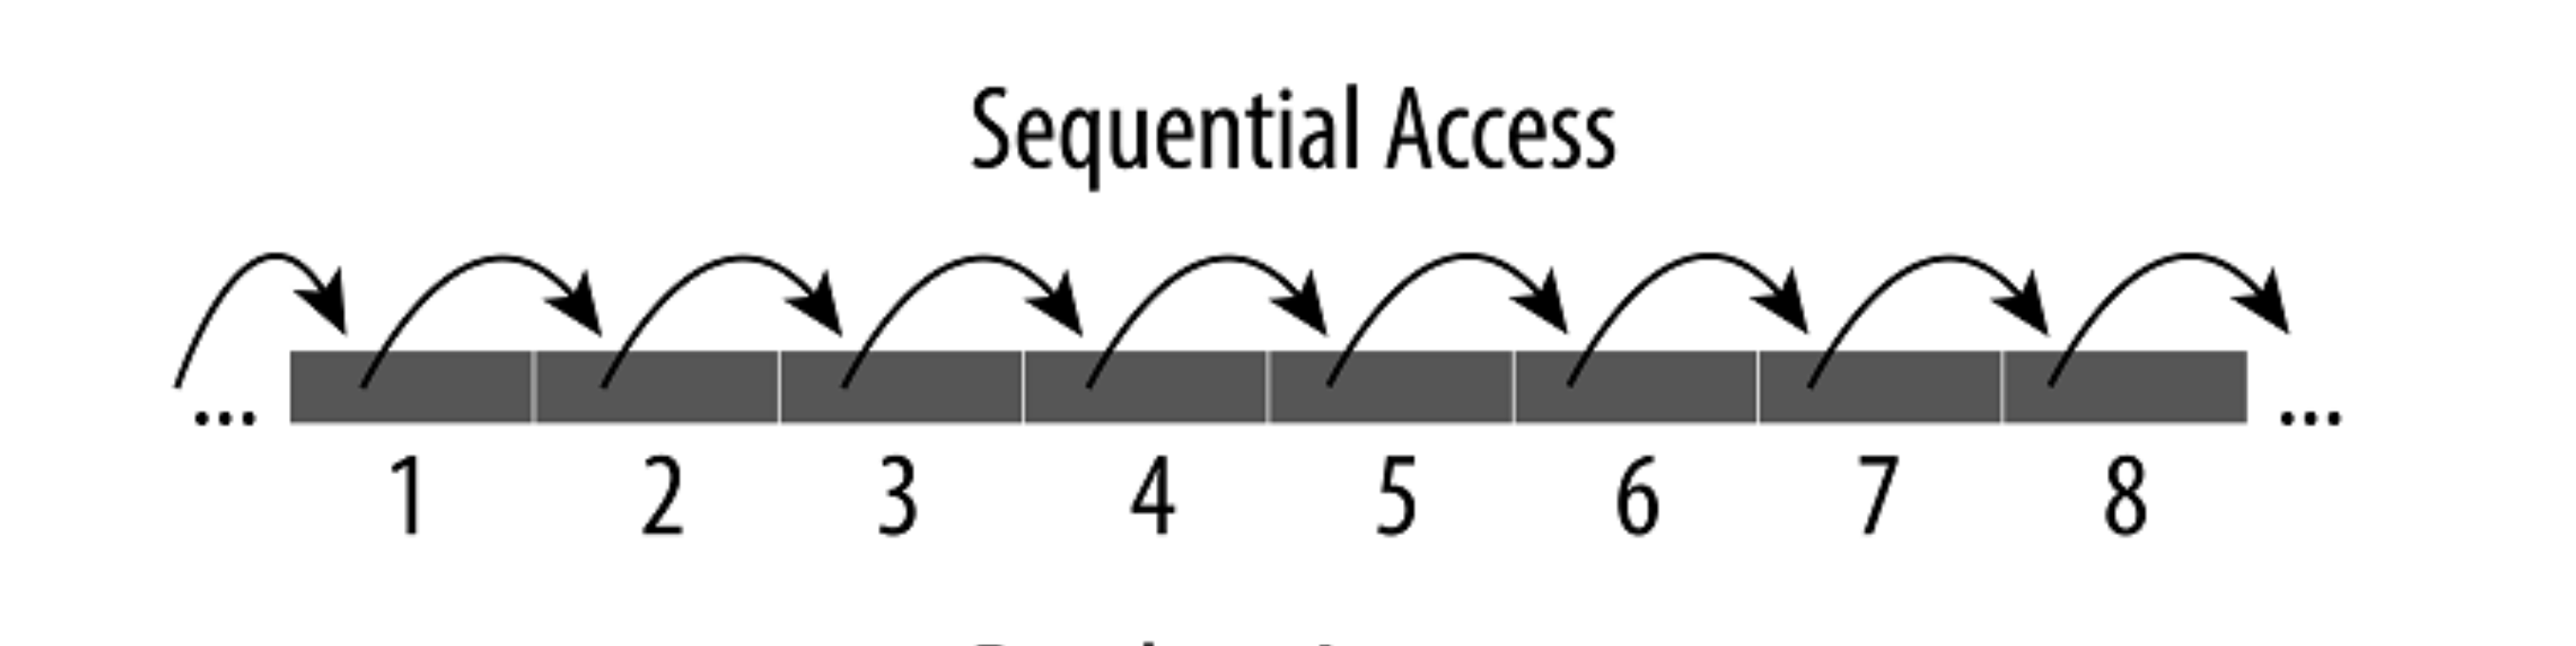
\includegraphics[width=6cm]{images/secuencial.png}
    \centering
    \label{fig:noaleatory}
    \caption{Acceso secuencial}
    \end{figure}

\subsection{Memoria de acceso aleatorio} Cada posición de memoria está organizada de tal manera que posee un único mecanismos físico de acceso, por lo que a diferencia del secuencial podemos acceder a registros de forma independiente. Esto permite eliminar el tiempo variable y acceder con el mismo coste cualquier registro independiente de su posición.

    \begin{figure}[h]
    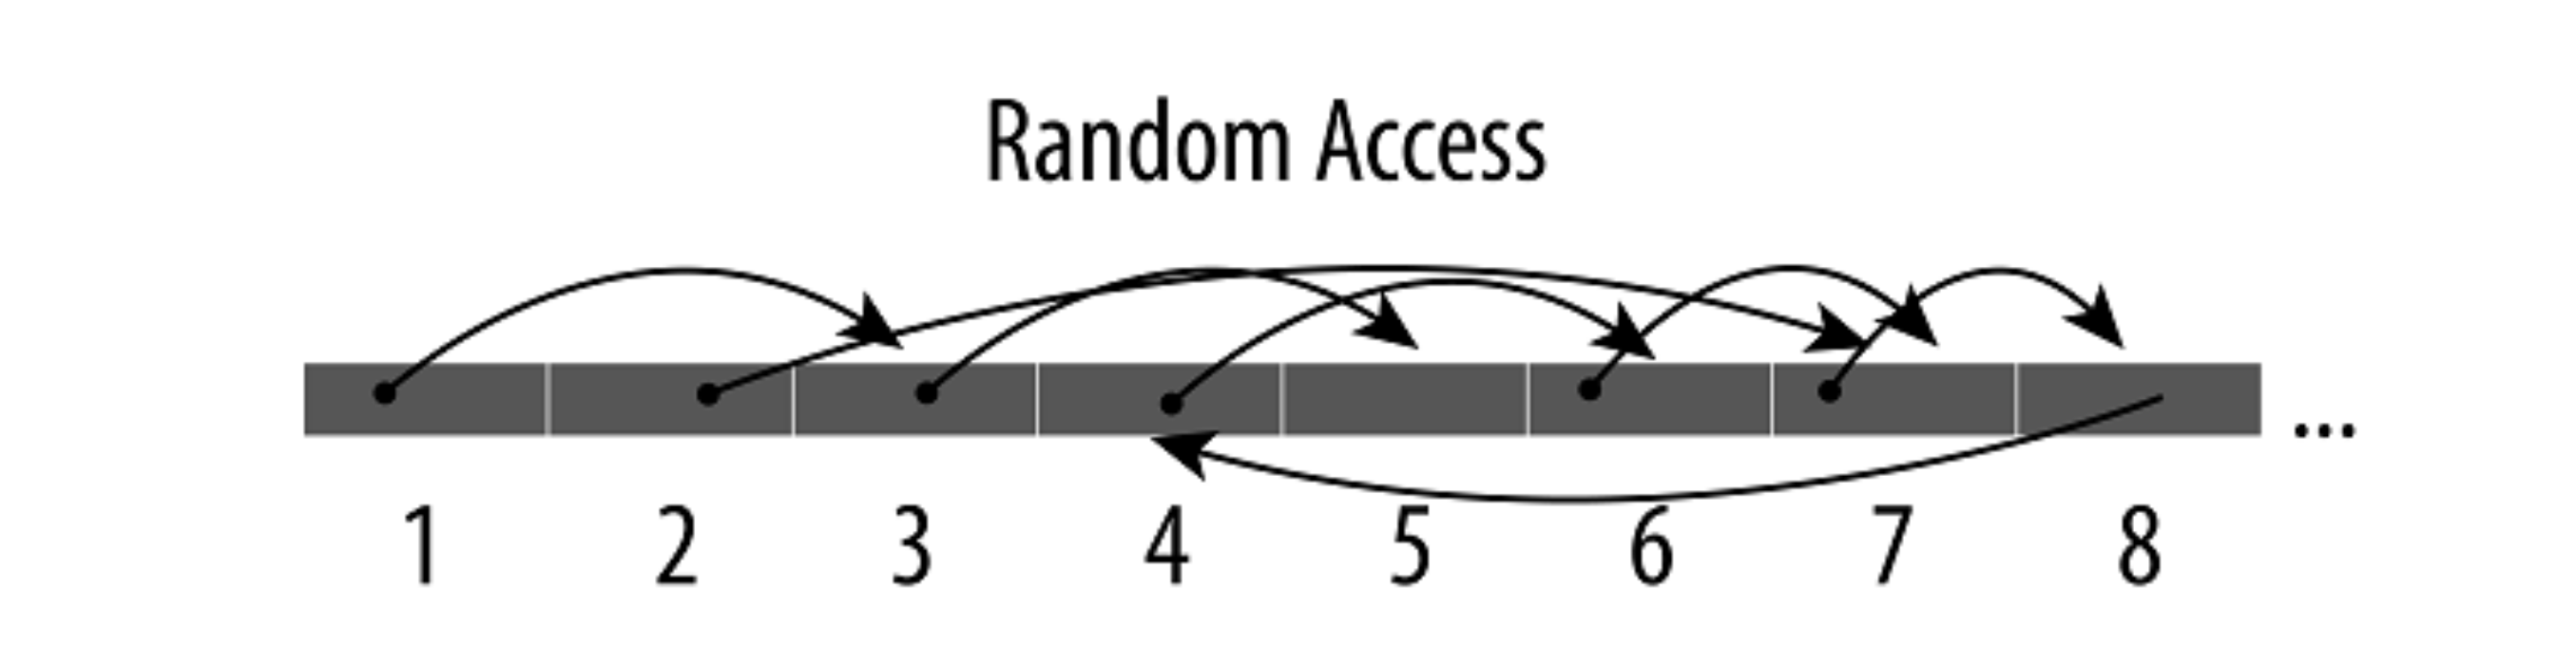
\includegraphics[width=6cm]{images/aleatorio.png}
    \centering
    \label{fig:aleatory}
    \caption{Acceso aleatorio}
    \end{figure}

\subsection{Memoria de acceso asociativo}
Este tipo de memoria conserva algunas características del tipo aleatorio. Además es capaz de hacer comparaciones de bits parciales teniendo parte del contenido a buscar en memoria, es por tanto una recuperación basada en porciones. Al igual que la memoria aleatoria tiene su mecanismo de direccionamiento y su tiempo de recuperación es constante.
Un ejemplo de ella es la \textbf{memoria caché}

\subsection{La memoria caché}
    \begin{figure}[h]
    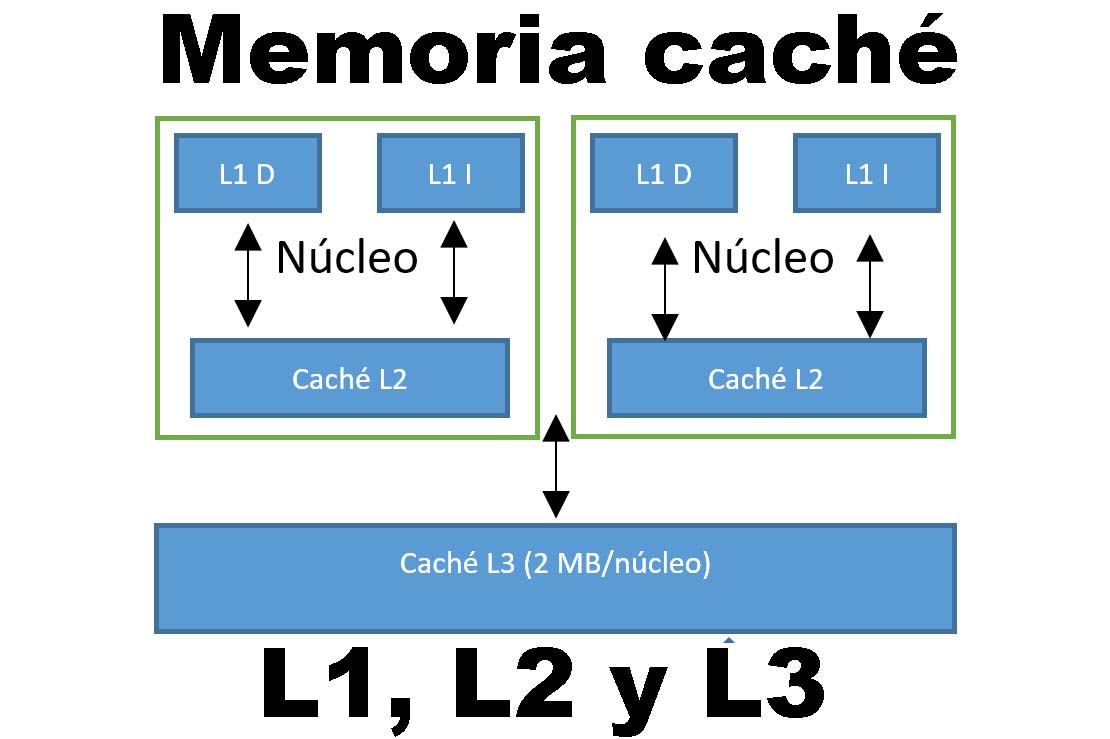
\includegraphics[width=6cm]{images/cache.jpg}
    \centering
    \label{fig:cache}
    \caption{Memoria caché L1 , L2 , L3}
    \end{figure}

La memoria caché se clasifica Desde L1 (teniendo un coste/bit alto) y descendiendo hasta L3 (coste/bit menor). Esta memoria está espacialmente más cerca del procesador y además presenta mayor velocidad de acceso que la memoria tipo RAM. Su función es facilitar el acceso de instrucciones 
 periódicas 
 para así disminuir la latencia que se experimenta al traer las instrucciones al procesador. Las instrucciones más usadas se almacenará en caché L1 y así hasta descender a caché L3.
(su tamaño comúnmente se clasifica en Megabytes)


\subsection{Read only memory (ROM)}
Se caracteriza por ser un memoria \textbf
{no volátil} por lo que sus datos son almacenados de manera permanente. Una ventaja significativa es que no requiere fuente de alimentación para memorizar los datos, su lectura es posible sin embargo no se puede escribir datos nuevos en ella. Suele usarse para cargar las primeras instrucciones de la máquina cuando se inicia para enterarla sobre la existencia de otros componentes.


\subsection{Dynamic Random Acces Memory (DRAM)}
La memoria de acceso aleatorio dinámica pertenece a la tecnología de memorias \textbf{RAM}. Conserva su características y consta de celdas que agrupa condensadores para representar de manera binaria los estados de sus condensadores (0 - 1). Naturalmente los condensadores presentan una tendencia a descargarse por lo que se deben recargar constantemente, de ahí que sea dinámica.

\subsection{Static Random Acces Memory (SRAM)}
La memoria de acceso aleatorio \textbf
{estático} al igual que las DRAM pertenecen a la tecnología \textbf
{RAM}, sin embargo su estructura de celdas no se basa en condensadores sino en transistores unidos entre sí(parecido al procesador) para formar una configuración cruzada y generar estados lógicos estables. La velocidad de este tipo de memorias es más rápida que la DRAM (aunque ambas necesitan refrescos periódicos al ser volátiles), al poseer un mecanismo más complejo requiere más espacio físico y por lo tanto su capacidad se ve reducida frente a su otra variante DRAM que consta de un circuito más sencillo y por lo tanto se pueden añadir más elementos en una placa
(estas memorias suelen usarse como caché al ser más costosa y las DRAM como memoria principal al ser más baratas y poseer mayor capacidad) es frecuente encontrar que la memoria principal que usan los computadores sea dinámica y no estática.

\subsection{Memoria de disco magnético}
Este tipo de memoria \textbf{no volátil} tiene su principal uso en el almacenamiento persistente. A diferencia de la memoria ROM la cinta magnetica permite escribir nuevamente los sectores y puede conservar su estado incluso cuando no tiene alimentación eléctrica. Algunas memorias de tipo magnetico son :

\begin{itemize}
    \item {Discos duros }
    \item {Memoria usb}
    \item {CD's}
\end{itemize}

Actualmente memorias como los discos duros se emplean para proveer almacenamiento permanente a las computadoras. Existen diversas limitantes para las memorias magneticas como la cantidad de revoluciones por minuto en discos duros tradicionales o la cantidad de veces que se puede sobreescribir los discos de estado sólido.
una caracteristica sobresaliente de este tipo de memoria es su alta capacidad de almacenamiento muy por encima de las tipo RAM.

\section{¿ Cómo se gestiona la memoria del computador ?}

La memoria está gestionada por el Centro de Control de Memoria (MCH
) cuya función principal es la de asignar el recurso de memoria además 
de liberar la memoria que no será usada por un proceso. También está encargado de gestionar los intercambios entre la memoria y el disco rígido.
Es importante aclarar que la gestión de memoria es tema de gran interés pues su optimización puede aumentar la eficiencia de la máquina.

\subsection{Unidad manejo de memoria (MMU)}
Cuando un programa legítimo quiere acceder a la memoria, la MMU
 se encarga de traducir la dirección virtual que maneja el kernel
 en una dirección física. Esta operación será comprobada para evitar el acceso de programas no autorizados a ella, de ser así se enviará una excepción al kernel
. Para llevar a cabo esto y evitar que se corrompa el sistema operativo o su ejecución, se almacena el límite de la instrucción más alta del S.O en los registros de la cpu. Cuando una operación intente acceder a dicho espacio será interceptada.

\subsection{Translation  Lookaside  Buffer}
Dentro de la MMU
 existe una memoria asociativa (muy similar a la caché
) cuyo objetivo es guardar datos que fueron accedidos recientemente. Cuando el procesador requiere la instrucción el TLB
 busca si tiene en su memoria dicho contenido,s ino emitirá un fallo y se procederá a buscar en la memoria.
\section{¿Qué hace que una memoria sea más rápida que otra? ¿Por qué esto es importante?} 

Cuando nos preguntamos la razón de que algunas memorias presenten mayor velocidad de transferencia es necesario aclarar algunos conceptos.Las memorias que integran tecnología basada en transistores (caché - sram
) poseé velocidades mayores precisamente por las características físicas de sus componentes en relación a la memoria común de condensadores. También influyen otros componentes encargados de la comunicación de esta misma, el \textbf
{BUS} (los circuitos que sirven de autopistas) entre la memoria y los microcontroladores pueden presentar cuellos de botella. Existe un problema conocido como latencia (tiempo de respuesta) que puede producir diferencias notorias entre las tecnologías de memoria.
La limitante física también está presente en los discos rígidos por ejemplo, estos deben alcanzar un numero determinado de revoluciones/minutos para acceder a la información y no generar retrasos considerables en la ejecución de algún programa.

Tener como prioridad conocer el funcionamiento del tipo de memorias existentes nos brinda la posibilidad de interactuar con ellas. Permite emplearlas de manera precisa en 
múltiples aplicaciones, conocerlas nos da la posibilidad de explorar sus limitantes y cómo estas pueden ayudarnos a resolver problemas específicos.
Entender el hardware nos ayuda a crear algoritmos óptimos que aprovechen los recursos existentes y comprender su rol en las máquinas modernas.
Nuestra sociedad cada vez genera más información, nuestras ambiciones necesitan más capacidad. Quizá en unos cuantos años las memorias que citamos acá solo serán parte de la historia. Para embarcarnos en ese viaje es necesario empezar aquí, conociéndo su funcionamiento ahora.
\bibliographystyle{IEEEtran}
\bibliography{references}
\cite{rebollo}
\cite{figura1}
\cite{ucm}

\end{document}
